
\section{Data Split} 
\label{sec:Data Split}


\begin{figure}[htbp]
  \centering
  \begin{subfigure}[b]{0.49\textwidth}
    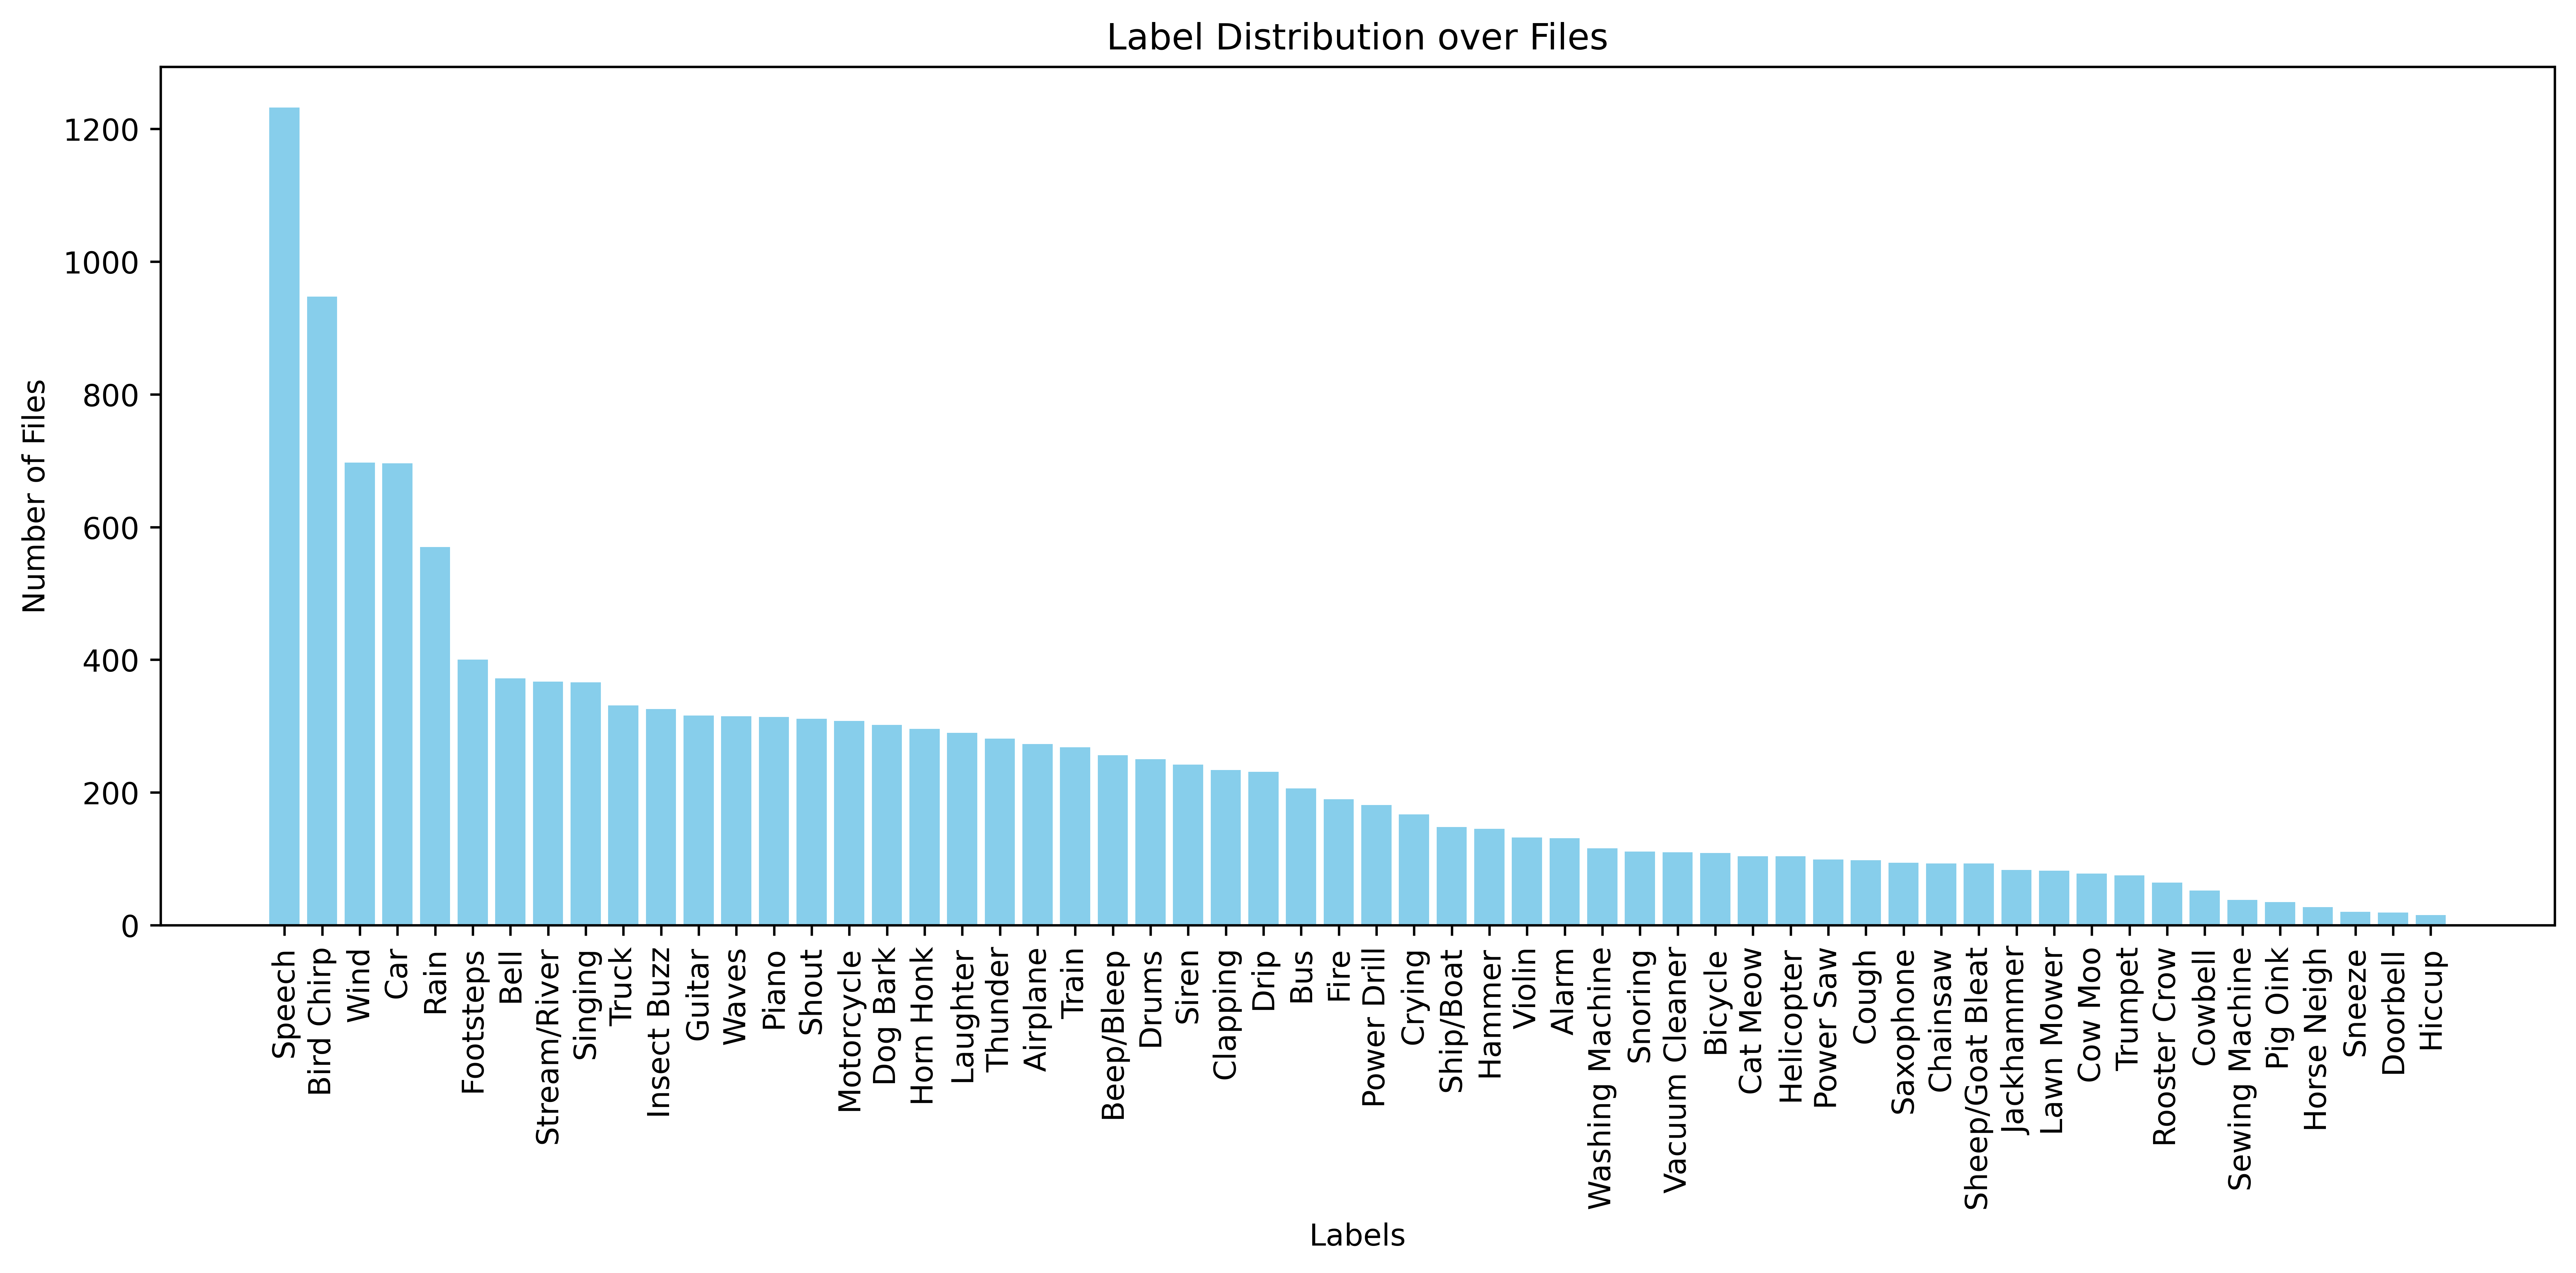
\includegraphics[width=\textwidth]{figs/2_Label Distribution over Files.png}
  \end{subfigure}
  \hfill
  \begin{subfigure}[b]{0.49\textwidth}
    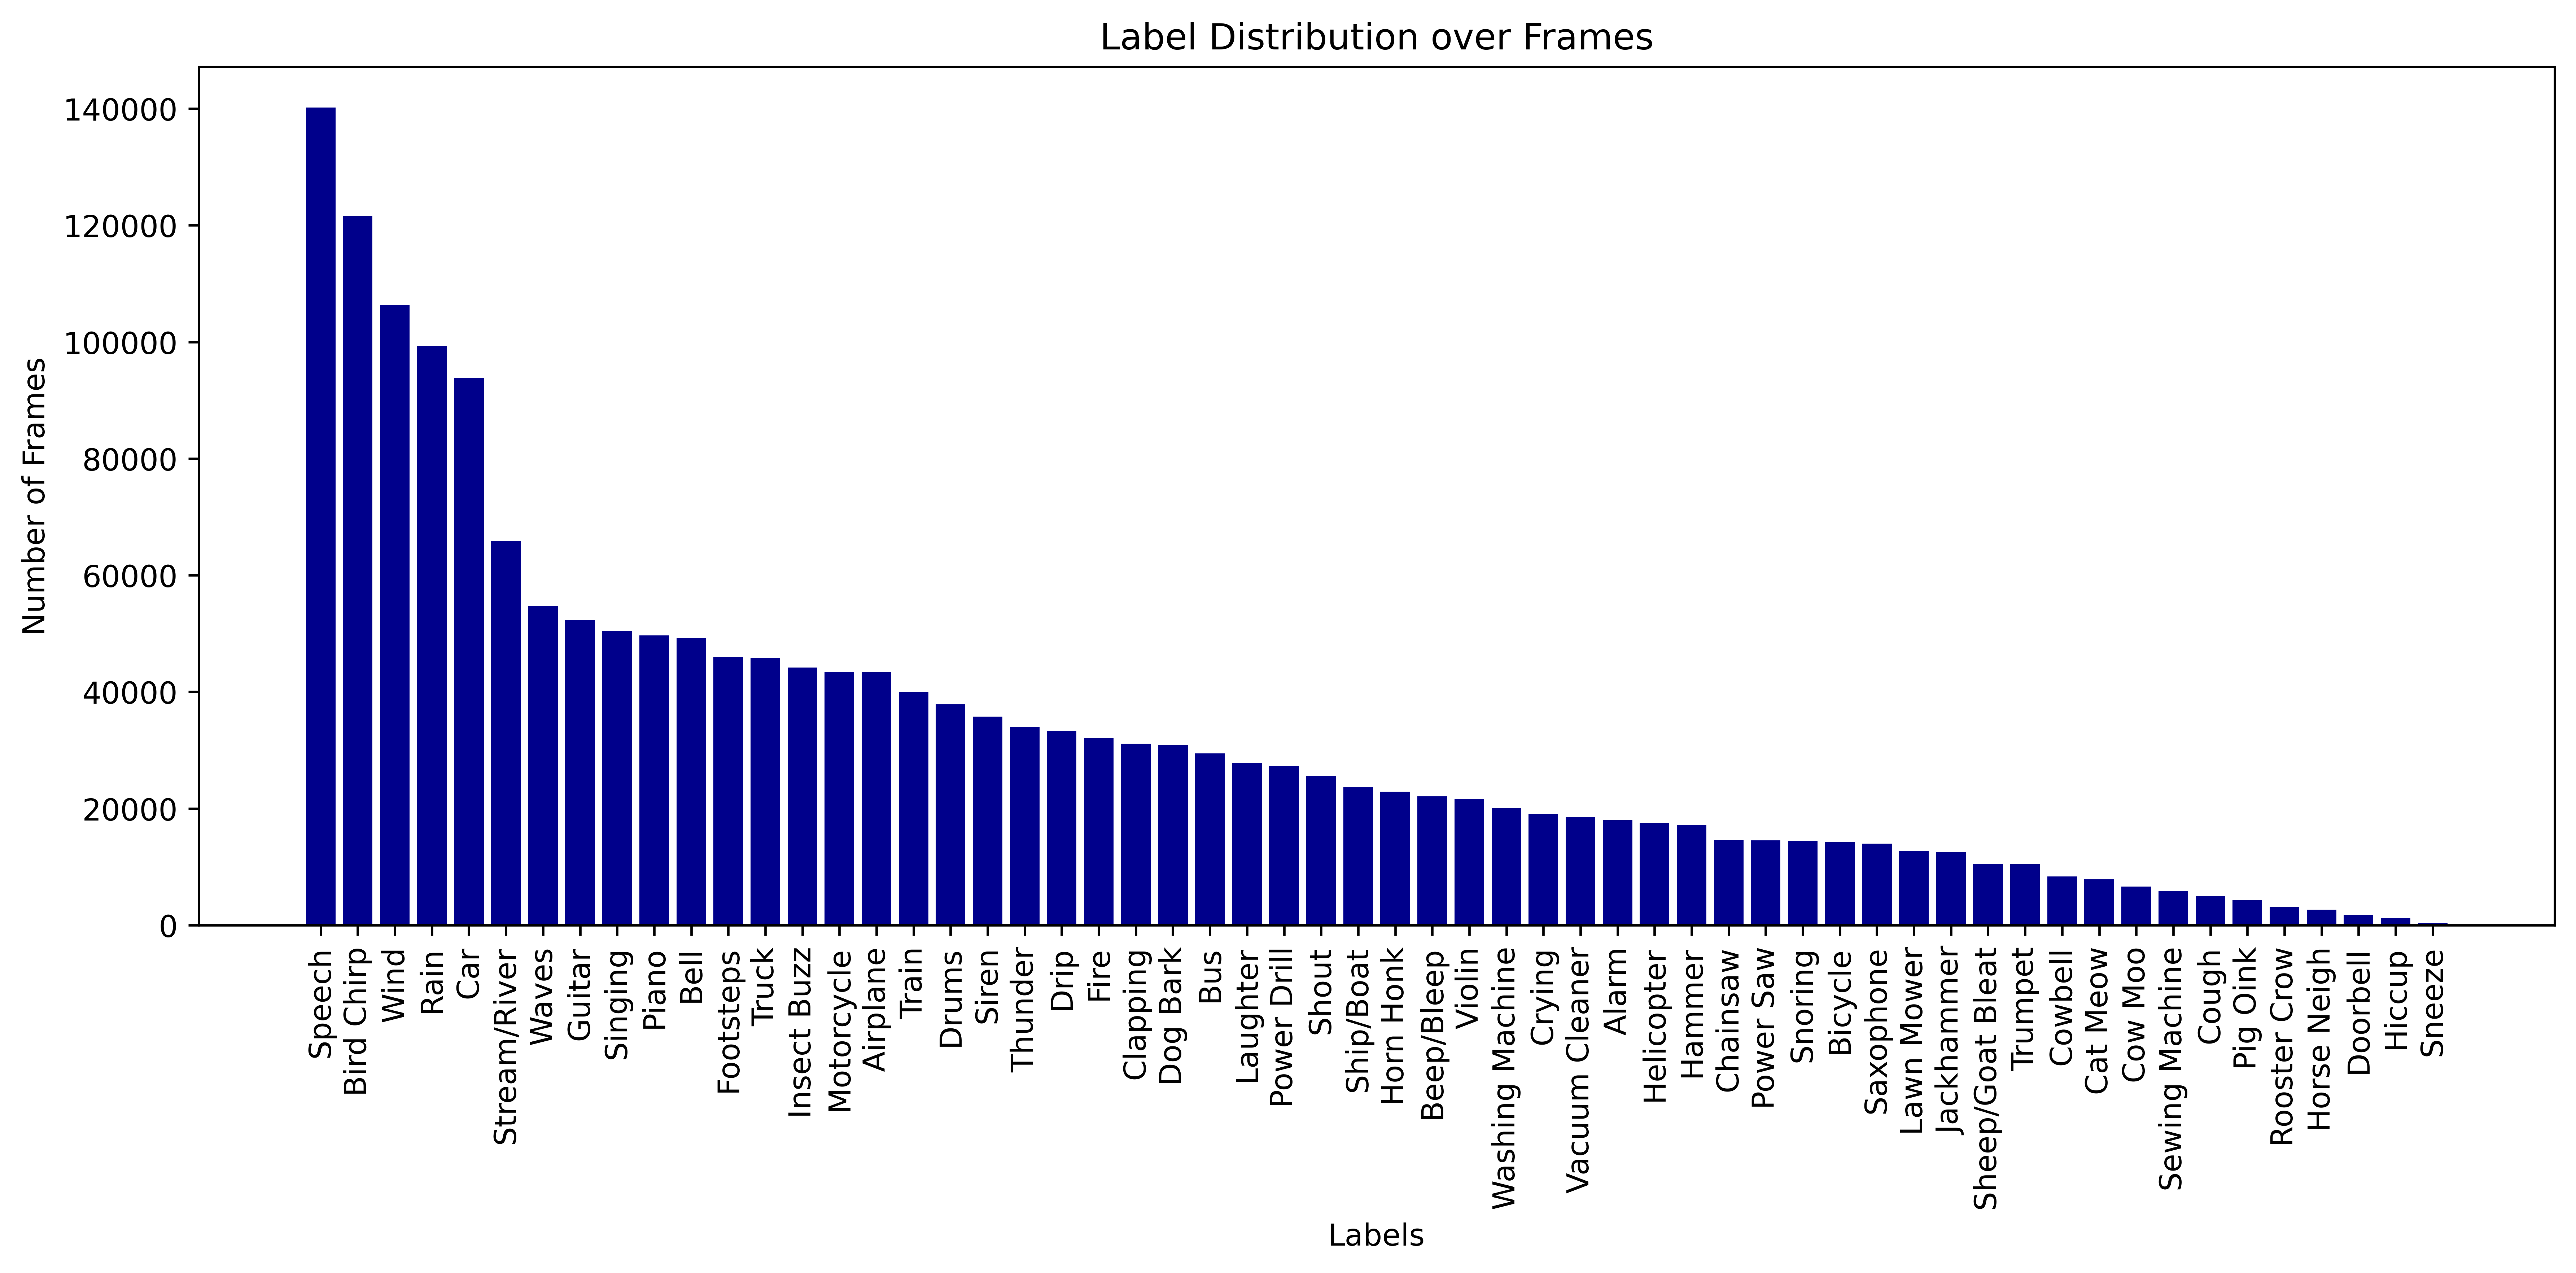
\includegraphics[width=\textwidth]{figs/2_Label Distribution over Frames.png}
  \end{subfigure}
  \caption{Label distribution}
  \label{fig:data-split}
\end{figure}



\subsection{Describe how you split the data for model selection and performance evaluation. }
\label{sec:Data Split:a}

For audio classification tasks, the standard and robust approach is to split the dataset into three distinct subsets to effectively train, tune, and evaluate the model:


\begin{enumerate}
	\item {\bf Training Set: } Used to train (fit) the model's parameters. Typically constitutes around 60–80% of the data. 60% in our case. 
	
	\item {\bf Validation Set: } Used for hyperparameter tuning and model selection. Helps prevent overfitting to the training data. Typically 10–20% of the data. 20% in our case. 

	\item {\bf Test Set: } Used only for final performance evaluation to estimate how the model will perform on unseen data. Hold back until the very end to provide an {\it unbiased final estimate of performance}. Typically 10–20% of the data. 20% in our case. 
\end{enumerate}

\begin{itemize}
	\item \uppercase{Alternative: } {\bf Cross-Validation} If the dataset is small, k-fold cross-validation (often with stratification) on the training+validation split can be used for more robust hyperparameter tuning. The test set remains untouched until final evaluation.
\end{itemize}


We first loaded all the audio data with the features and the labels and split it into individual frames. 




\subsection{Are there any potential factors that could cause information leakage across the data splits if they are not carefully designed? If yes, how did you address these risks?}
Yes, there are {\bf critical risks of information leakage} in audio classification if splits are not carefully designed:


\label{sec:Data Split:b}

\begin{itemize}
	\item {\bf Common Sources of Leakage: } \\
		{\it Overlapping audio segments: } If data is split by segment but not by full recording/file/session, temporal leakage can occur. \\
		{\it Same noise/audio source in multiple splits: } If one noise/audio source appears in both training and test sets, the model may learn source-specific features rather than class-specific ones. \\
		{\it Similar background noise or recording conditions: } If recordings from the same session or environment are in multiple splits, the model may overfit to irrelevant cues. 
	
	\item {\bf Mitigation Strategies: } \\
		{\it Source-Independent Splits:} Ensure that all data from a single noise/audio source is assigned to only one of the training, validation, or test sets. \\
		{\it Session-Based Splits:} If the data includes session or recording metadata (labels), use it to group and split accordingly. \\
		{\it Careful Preprocessing:} Avoid any preprocessing (e.g. feature normalization) that uses statistics from the full dataset — use only training data statistics. 
\end{itemize}


To avoid possible problems when splitting into the three data sets, 
we only split at file boundaries and tried to have an approximately equal distribution in all parts (stratification)  (\hyperref[fig:data-split]{Figure~\ref*{fig:data-split}}).
We worked in frames during pre-processing (normalization).




\subsection{Describe how you obtained unbiased final performance estimates for your models. }
\label{sec:Data Split:c}

To ensure the final performance estimate is unbiased:

\begin{enumerate}
	\item {\bf Strict Test Set Separation: } The test set is never used during training or validation. Final model evaluation is performed only once on this set after all model development is complete.
	
	\item {\bf Validation-Driven Tuning: } Hyperparameters and model architecture are selected using only training and validation data. 
%		If cross-validation is used, it’s done within the training+validation data.
%	
%	\item {\bf Repeated Experiments: } If randomness (e.g. in weight initialization or data sampling) affects results, the experiment is repeated with different seeds and the average + standard deviation is reported.
%
%	\item {\bf Stratified Sampling: } Ensures that the class distribution in all sets reflects that of the full dataset, which is particularly important in our case (unbalanced data sets).
\end{enumerate}




